\chapter{Object Recognition Approach}\label{ch:obj_rec}
To recognise an object in an image, different methods of object recognition can be used. In this chapter three methods are presented: edge, shape and colour recognition. Where edge and shape covers different methods used for actual recognition, colour recognition introduces aspects that must be considered if the recognition is done on colour images.

A universal trait for edge and shape recognition is that there are many different implementations for each of them. The following section, "\nameref{sc:com_vision}" in \ref{sc:com_vision}, describes the common issues with image analysis. Following this, the general concepts of egde and shape are described and the aspects of colour is introduced.  After the introduction of edge, shape and colour recognition, it is decided in \cref{sc:obj_final} which methods to use and how to perform the actual recognition. The chapter is based on the book "Image Processing Analysis, and Machine Vision" \cite{obj_recogn_book} and supported by the article "Shape recognition with edge-based features" \cite{shape_recogn}.

\section{Computer Vision}\label{sc:com_vision}
The field of computer vision looks to mechanically duplicate the sight of a human, including how vision is perceived and understood.
Many difficulties are connected to computer vision. This section introduces a subset of these. In extension, it is the same problems that are connected to image analysis and thereby object recognition in general. It is because of this connection that the problems are covered.

\subsection{Dimension Transformation}
When an image is captured, the 3D world that humans see is transformed into a 2D space. As a result of this, properties such as depth and actual size is lost. Thus, small objects close to the capturing device can seem as big as large objects placed further from the capturing device.

\subsection{Interpretation}
The human mind is able to see a new setting in an image and reason about its content. An example could be that we can recognise a river in a image regardless of the dimensions and flow of the river. A computer is not able to do the same recognition without support. One way to support this feature is by using \gls{ai}, which can learn from some settings and recognise new settings which furthermore can be used to expand its knowledge base.

\subsection{Noise}
Noise in images includes a dusty lens that causes white noise, poor focus, as it also can be caused by too little or too great illumination. Noise can have a negative impact on the result and is difficult to avoid, hence mathematical methods have been developed to cope with noise, but this makes image analysis more complex if included.

\subsection{Big Datasets}
The greater the quality of images the larger the size of the data. Furthermore, if working with a stream of data eg. streaming a certain amount of frames per second, the amount of data can quickly become much greater. This in turn can have a negative impact if working with real-time systems, as the data will take longer to analyse. 

\subsection{Brightness}
Shadows in an image can influence how similar objects are presented and analysed, an example being that a colour in a shaded area can seem much different if it is in a bright area. Other aspects that can change how the image can be interpret are the direction of one or more light sources, and the surface structure and reflective properties of objects in the image.

\subsection{Local and global view}\label{ssc:loc_glo_view}
One of the reasons it is complex to recognise objects with machine vision is because of the input domain of the used algorithms, as they are designed to analyse a local area, such as a pixel and it's neighbourhood, much like looking through a keyhole. With only a few keyholes any object can become difficult to recognise, even for the human mind. This could possibly be solved by creating algorithms which can analyse from a global view, but this includes the use of \gls{ai} and covers an area in that field, in which it has been argued that a formalisation context is crucial in making the needed generalisation, but formalisation of eg. complex shapes is a very difficult task. Hence making the dependencies for implementing \gls{ai} just as difficult. \citep[page 5]{obj_recogn_book}
\section{Edge Detection}
Edge detection, as the name implies, attempts to detect edges in an image. This can be done in many different ways, some of which are introduced in \cref{ssc:edge_preprocessing}, \nameref{ssc:edge_preprocessing}. However, to use edge detection for recognition, the detected edges needs to be described in some way for recognition algorithms to understand the data. Methods to perform this description are presented in section \cref{ssc:edge_based_segmentation}.

\subsection{Preprocessing}\label{ssc:edge_preprocessing}
Preprocessing covers the detection of edges and is needed before edges in an image can be described and analysed. The preprocessing detects edges to determine certain properties. This is done with operators, some of which are described in the following. Furthermore, other aspects have influence on detecting edges. These aspects are mentioned after the introduction of the operators.

\subsubsection{Operators}
Preprocessing includes a number of operators which calculates gradient for a given pixel. Gradient defines how an image is changing in regards to colour or illumination. The gradient is defined by two aspects, gradient magnitude and gradient direction. Magnitude is the rate at which the change is happening, and direction tells in which direction the illumination or colour levels rises. The direction has offset in the horizontal axis, meaning a direction to the right is 0\degree. The degrees then follow the rotational direction which is counter clockwise, as an example 180\degree is directly left.
 
In order to gather the gradient information, it is not enough to look at each pixel alone, therefore most operators work with a 3x3 mask, which is a region of 9 pixels. The center pixel is the pixel of interest and the surrounding pixels are used for references.

Since pixels are to be analysed, there must exist a way to identity each pixel. Images are often split up like coordinate systems, where each pixel has a unique coordinate, annotated $(x,y)$. X is the horizontal position and y is the vertical position. The offset for the enumeration is in the upper left corner, so the upper left pixel is denoted $p=(0,0)$, whereas the bottom right pixel is denoted $p=(x_{max}, y_{max}) $.

The operators are designed to compare pairs of pixels around the chosen pixel. The operators either look in a \textit{4-neighbourhood} or \textit{8-neighbourhood}. For a 4-neighbourhood it means the operators solely look horizontally and vertically, using the pixels left and right of the center pixel, and directly above and below the center pixel. The 8-neighbourhood looks in the same directions as the 4-neighbourhood, and in addition to this it looks on the diagonal pixels.

\textbf{An example}

The following example serves to illustrate the use of mask and gradient.
Consider an image that is ½ white and ½ black, with the white half at the top of the image. In most gray-scale images, white is fully bright and black is of no brightness\citep{gray_scale_brightness}. This means white has a value of 255 and black has a value of 0. If looking at a black pixel on the border between the black and white, the gradient direction is 90\degree\ as the gradient levels increases in a north direction, which corresponds to 90\degree. The 3x3 mask is placed with the pixel in the center. The gradient magnitude can then be calculated by the formula $mag(x,y)=\sqrt{dy^2+dx^2}$. $dx$ is calculated by subtracting the pixel to the right of the center-pixel with the pixel the the left of the center pixel, and $dy$ is calculated by subtracting the pixel above with the pixel below. 

Calculating $dx$ and $dy$ will in the example yield $dx=0-0$ and $dy=255-0$, so there is no change in the horizontal(x) direction, which follows the border. There is, however, a big change in the vertical(y) direction, which makes sense because the pixel is on the border between white and black.

\textbf{Laplacian operator}

The laplacian operator calculates the magnitude of pixels. It can be used when the gradient magnitude is the only value of interest, as it does not take any regards for direction. It is often used with the aforementioned 3x3 mask and can be used to look either in a 4- or 8-neighbourhood. One disadvantage is that it looks twice at some edges.
The Laplacian operator is often used for image sharpening, which is intended to sharpen edges to be more visual for the human eye.

\textbf{Compass operators}

A specific subset of operators is called compass operators as they estimate the gradient direction together with the magnitude. All the operators work with a 3x3 mask, and some allow larger masks to be used. Most operators calculate gradient magnitude for all pairs of opposite pixels in the border of the mask and the greatest magnitude then defines the gradient direction.
In addition, some compass operators define the direction by three pixels in each direction, where the gradient magnitude for the negative direction(towards darker areas) are negated, as illustrated in \cref{fig:mask_dir}.
Some operators differ in the way that they utilise all eight pixels in the mask border to define the gradient direction, where three pixels are used for negative direction(illustrated with -1) and five for the positive direction. Another difference is an operator which also marks direction by three pairs of pixels but the operator only detects horizontality or verticality of edges. This means that the resulting image for horizontality only has horizontal lines, and vertical lines are drawn using short horizontal edges, over the span of the vertical line, and horizontal lines will appear as is, and vice versa for verticality.
\begin{figure}[H]
	\centering
	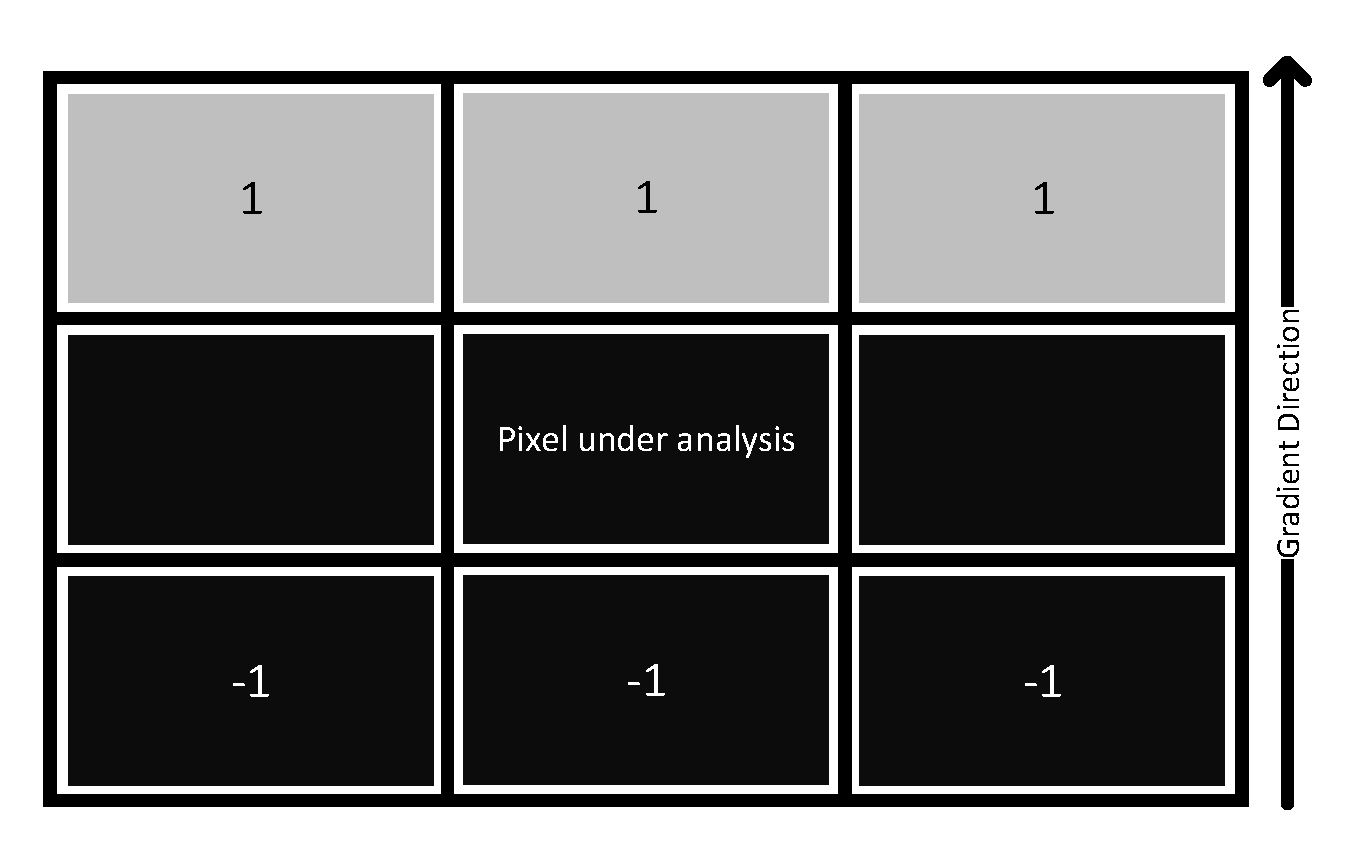
\includegraphics[width=0.5\textwidth]{graphics/mask_directed.pdf}
	\caption{Weighted values corresponding to gradient direction}
	\label{fig:mask_dir}
\end{figure}

\subsubsection{Scale}
Most image analysis methods, including edge detection, works locally. Increasing the scale gives a larger locality, as the analysed neighbourhood is increased, which in turn can give more precise estimates. However, the neighbourhood can also become too large and detail is lost, as some edges can be ignored either because of noise from other segments or because the details themselves are seen as noise.
If a large scale or possibly a global scale is to be used, the same problems of implementing \gls{ai} as mentioned in \cref{ssc:loc_glo_view} will occur. The optimal scale when working locally varies across the analysis of an image, as some parts might need more details to be captured, and some parts like a thick edge would need more scale to be recognised correctly.

\subsubsection{Edge profiles}
Edge detection can be improved by applying an edge profile, which defines the type of edges that is searched for. Two such profiles are illustrated in \cref{fig:roof_profile} and \ref{fig:step_profile}. The roof profile \cref{fig:roof_profile} is often used when detecting thin lines, whereas the step profile \cref{fig:step_profile} can be used in situations where there is a great difference in a region and the surrounding region.
\begin{figure}[H]
    \begin{minipage}{0.5\textwidth}
    	\centering
    	
\includegraphics[width=0.80\textwidth]{graphics/roof_profile.pdf}
    	\caption{Roof profile}
    	\label{fig:roof_profile}
    \end{minipage}%
	\begin{minipage}{0.5\textwidth}
    	\centering
    	
\includegraphics[width=0.80\textwidth]{graphics/step_profile.pdf}
    	\caption{Step profile}
    	\label{fig:step_profile}
	\end{minipage}
\end{figure}


\subsubsection{Multi-spectral images}\label{ssc:m-s_images}
The edge detection described so far covers images in a single spectral range, such as grayscale images. Multi-spectral images includes RGB images and light frequencies out of the human visual range, such as infra-red. When working with multi-spectral images the different spectral bands must be analysed, for RGB, meaning the red, the green, and the blue spectral bands. This can be done in various ways, one of which is to analyse edges in each individual spectrum and combine the partial results for a final result. Other methods include using the difference of gradients between two spectres or using a multi-spectral edge detector which uses gradient information from all spectral bands.

\subsubsection{Edge Detection Using Threshold}\label{ssc:edge_threshold}
Threshold is an old technique for segmenting objects and background mainly in grayscale images. It is inexpensive and fast to execute but works best if objects are separated and there is a distinct difference in the brightness levels of the objects and their background. Choosing a proper threshold value is a necessity for a correct segmentation, as a low threshold will lose segmentations and a high threshold will include too much information.
Furthermore, a single threshold is rarely enough for an image. Often there are both lower- and upper-bound values, but the optimal segmentation value can also vary across an image. As mentioned, threshold segmentation is mainly used for gray-scale images, but can also be used in multi-spectral images in the same ways as explained in \cref{ssc:m-s_images} for multi-spectral images.

\subsection{Edge-based segmentation} \label{ssc:edge_based_segmentation}
The edge detection methods described hitherto detect edges and cannot solely be used for describing edges and borders in an image. So far each individual pixel has been analysed to see whether this pixel can be part of the edge of an object. The next step is to connect the edge pixels, while also keeping in mind some of these might be noise. Describing edges covers ways to specify how edges are to be interpreted in an image. Two separated circles on a uni-coloured background must be described as separate circles. Different edges on the border of each circle must be connected such that the circle can be described as a whole. This results in two circular segments with the background being a third segment. There are different ways to perform such a segmentation. The rest of this section explains how the segmentation can be done based on the edges that has been detected.

To do this segmentation, other methods can be applied for combining detected edges into edge chains that corresponds better with actual lines in the image. An edge chain contains information to describe how edges are connected to each other. One way to do this notation is to use numbers 0-7 to specify a direction, where 0 is right, 1 is upper right, 2 is up, and so on.
Using an edge pixel as reference, the chaining can then begin by noting what position the starting pixel is in, and noting what direction the next edge pixel is. If the chain at some point arrives at the reference pixel again, a complete segment has been found. This chaining can then be done for all edges.

Another method for edge-based segmentation is \textit{edge relaxation}, which analyses a central edge that is an edge in the crack between two pixels, illustrated with features on \cref{fig:crack_edge}. The central edge is connected to three cracks on each side and with knowledge from these six cracks, edge relaxation is able to determine if the central crack edge is part of an edge border.
The belief of the crack edge being a border edge is denoted by a confidence level, which depends on the information gathered from neighbouring cracks. For example, if neither of the neighbouring cracks are believed to be border edges, then the belief of the central crack edge to be a border edge is zero. If some of the neighbouring cracks have edges, then the confidence that the central crack edge is a border edge is raised. To extend this method, two other crack edges parallel to the central crack edge can be added as competitors to which the central edge must have a greater confidence level.

\begin{figure}[H]
	\centering
	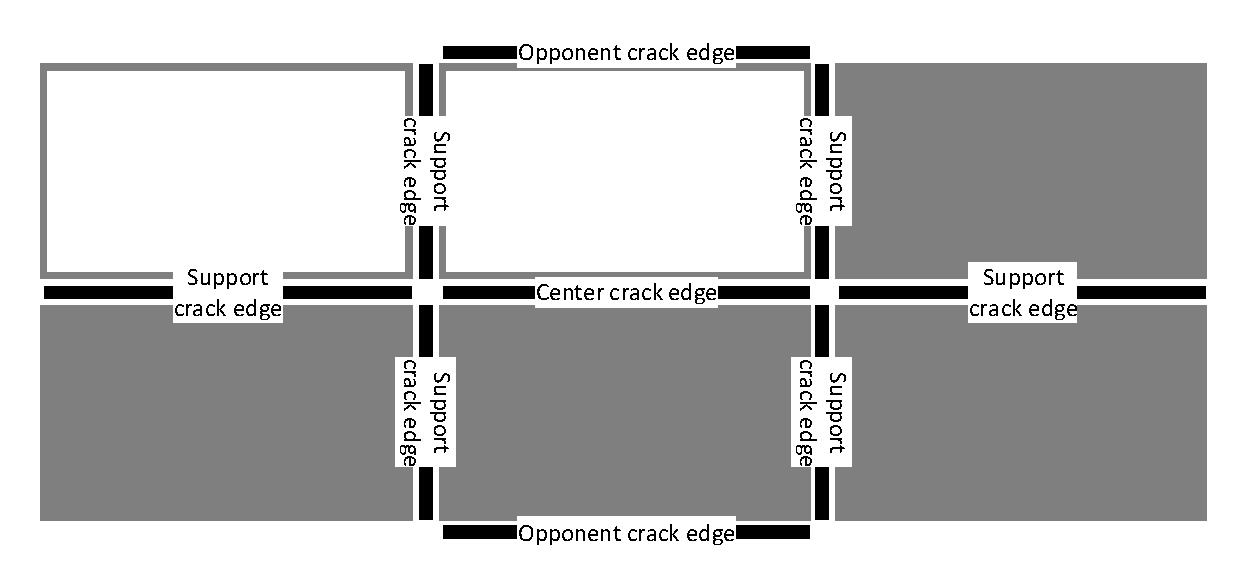
\includegraphics[width=0.5\textwidth]{graphics/crack_edges.pdf}
	\caption{Illustration of crack edge and supportive features}
	\label{fig:crack_edge}
\end{figure}

The methods described so far detects borders which partially or completely segments the given image. If this segmentation is complete, the edges outline all the regions in the image. However, if some borders are partial, the determination of regions is  complex, as it often requires higher-level information about the object, such as shape and size. Even with this information, the partial regions might not be acceptable; several regions can be blurred together and seen as one. A method of determining regions from the partial segments is to compare segments from different threshold values. Another method which includes the gradient direction considers a closest opposite edge pixel, by searching in a straight line which may have a maximum distance \textit{M} between them following the negative gradient direction of border pixel, a simple illustration is shown in \cref{fig:partial_region}. If two edge pixels can be connected this way, those two and all pixels in the line between them are marked as region members. If a pixel gets atleast three marks, it is considered a region member, otherwise it is marked as a background pixel. The \textit{M} distance is often chosen from knowledge of the size of the regions of the object that is of interest.

\begin{figure}[H]
	\centering
	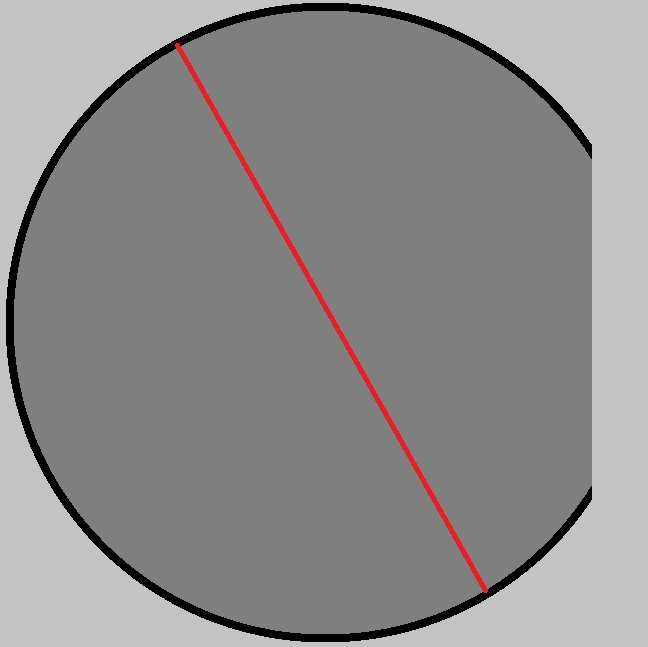
\includegraphics[width=0.5\textwidth]{graphics/partial_region.jpg}
	\caption{Simple illustration of opposite pixel pair in partial region}
	\label{fig:partial_region}
\end{figure}
\section{Shape Recognition}
This section describes some of the general issues with shape recognition, and introduces methods to perform shape recognition. Edges are also used in this section, but to distinguish edges in edge detection from edges in shape recognition, the edges in this section will be referred to as contours.
Shape recognition is seen as a difficult task, the reason being that both simple and complex shapes have not yet been precisely described in computer vision. This is a necessity for giving generalised descriptions of shapes\citep[page 328-329]{obj_recogn_book}.
Scale is also a big issue, as high resolutions can result in noise in regards to contour detection.
Furthermore, low resolutions can result in the loss of small details. One way to minimize the issues that scale can give, is to recognise shapes at different resolutions. However, this is more complex, as it requires corresponding shape representations for each resolution.

Despite the difficulty of shape recognition it is still used in various fields. This experience cannot be used for generalizing because the fields use it in different ways, but a set of characteristic can be defined from this experience, and are often considered when planning to perform shape recognition. The characteristics include the following:

	\textit{Input representation form:} Object descriptions can be based on region boundaries or in a more complex manner with knowledge of whole regions.

	\textit{Object reconstruction ability:} If an object's shape can or cannot be reconstructed from the description.

	\textit{Incomplete shape recognition ability:} To what extent an object can be recognised if occluded by other objects, or other reasons for which only partial shape information is available.

	\textit{Local/global description character:} The global description can only be used if there is complete data of the object. The local description characterizes object properties from partial information, which also makes it usable for occluded objects.

Shape detection works with regions, which can be described in different ways, mostly from contours with properties. One way to gain information about these properties is with the use of edge detection.
There are numerous ways to describe the borders of regions which is mostly done in coordinate systems. \textit{Polar} coordinates is one such way, where border elements are represented as pairs of an angle and some distance.
A necessity for region description is to have region identification. This can be done in a number of ways, including enumerating each region. This way the total number of regions is equal to the greatest identification number. Another way is to use as few numbers as possible, and simply make sure no two adjacent regions have the same number. Four is the theoretical maximum needed to note regions with this approach. If the enumeration has been done this way, it requires one iteration over all regions to count the total amount of regions in the image.

There are two main ways to perform shape recognition. Being either contour-based or region-based,  both these options include various methods and are introduced here, .
\subsection{Contour-Based Shape Representation And Description}
One way to do contour-based shape representation is by \textit{Boundary description using segment sequences}, which represents boundaries(closed borders) by segments using specific properties. A linear line segment can be defined by two points $x_1$ and $x_2$ on the contour. This line can be mangled to follow the contour more, if it does not satisfy some pre-set requirements. One such requirement is the \textit{tolerance interval approach}, where a tolerance distance is defined for how far the contour between the two points may be from the line segment. If the tolerance distance is exceeded, the line segment must be split. A simple way to do this is by searching for the point that is furthest away from the line segment. At that point on the line a new point for the line segment is added, and a new chain of line segments is defined as $x_1 \rightarrow x_3 \rightarrow x_2$.

Another boundary segmentation is \textit{constant curvature} where second order polynomials are used to describe the possible structures that the line segments can have. The issue of scale mentioned in the beginning of this section also applies for these methods, as segmentation of curves can differ across both higher and lower scales. There is however, a \textit{scale-space} approach which ensures that detail is not lost and that new segmentation points only appears at greater resolutions \Citep{obj_recogn_book}.

\subsection{Region-Based Shape Representation And Description}
Boundary information makes it possible to describe regions, which in turn makes it possible to describe shapes, which is the goal of this kind of shape description. A large set of heuristic approaches to shape description can be used to describe simple shapes such as a circle or square. However, to describe more complex shapes, such as non uniform shapes with holes and a wrinkled contour, other methods must be used. One such method is region decomposition which splits regions into sub-regions that may be simple shapes. These simple shapes can then be described. When using region decomposition, the objects are represented by a planar graph, where no edges cross each other. The nodes represent the sub-regions resulted from decomposition and the edges represent the neighbourhood relations.
Furthermore, the region shape is lastly described by graph properties, the reason for this being that there is a number of advantages from graph representation, eg; being insensitive to small shape changes, it is fast to search through to gather information and it can be easily visualised.

\subsubsection{Heuristic Shape Descriptors}\label{ssc:heuristic_descr}
To do region decomposition, it is necessary to describe sub-regions, some basic descriptors can be used to do this, these descriptors include the following:

\textit{Area} is the simplest and most natural descriptor, given by the number of pixels in the region.

\textit{Euler's number} which is given by $\vartheta=S-N$ where S is the number of contiguous parts of an object and N is the number of holes in the object. An object can consist of more than one region, but if it only consists of one region then S=1.

\textit{Projection} is another descriptor which can be defined in any direction, eg. horizontal and vertical. The projections are binary representations of the pixels. If one row is of a length of seven but there is a hole of two pixels in the middle then only five pixels are projected and the hole does not exist in the projection.

\textit{Compactness} is defined by $compactness=\frac{(RegionBorderLength)^2}{area}$. The most compact shape according to this definition is a
circle, as it has the largest possible area in respect to border length. Compactness in digital images is defined by an inner boundary in the interval $[1,\infty]$.

\subsubsection{Region Decomposition}
As previously mentioned, region decomposition splits regions into sub-regions of simpler shapes. The idea of region decomposition is based on shape recognition being a hierarchical process. The first step is to decompose the region to get the subregions, representing simple primitive shapes. The second step is then to analyse these primitives, which can be done with the aforementioned heuristic shape descriptors in \cref{ssc:heuristic_descr}. The sub-regions can be noted as primary sub-regions, which can overlap to have the entire region described. The sub-regions can be represented as a graph, furthermore, if the sub-regions are represented by polygons, and not just line segments, graph nodes may carry informations which in turn can be used to specify properties, including if sub-graphs are rotation and size invariance.

\subsubsection{Region Neighbourhood Graphs}
A benefit from region-based shape recognition, is that it can be described by the use of graphs. With knowledge gathered from region decomposition, either through image decomposition into regions, or region decomposition into sub-regions, the graph can be presented as a region neighbourhood graph. This graph represents every region as a node and nodes of neighbouring regions are connected by edges. In addition, the relative position of two regions can often be used in a description process. However, simple notions such as "being left of" can be ambiguous and must be explicitly defined. For example, "being left of" can be defined as "The center of gravity of A must be positioned to the left of the leftmost point of B and the rightmost pixel of A must be left of the rightmost pixel of B".
\section{Colour Recognition}
Colours have been used by humans in a long time to perceive reality, whether it is through paintings, television, etc. But humans are still not able to express colours in absolute terms, and instead use terms like "London-telephone-box-red" to describe certain nuances of colours, or near the absolute colour with estimations as "the bottle has a green'ish colour".
When working in the field of computer vision, there is the advantage of cameras which can be used as a measurement units and cameras does measurements in absolute quantities. So the "green'ish" colour would be specified with a value which can be replicated exactly.

Colours can be measured as wavelengths. Some colours, such as low frequency ultra violet and high frequency infrared colours, are not part of the human visual spectrum, and therefore requires specialised tools for humans to see. The human visual spectrum is a narrow part of the total colour spectrum, and is approximated to be between 380 nm and 740 nm.
The human visible colours can be represented as a combination of primary colours and there is a number of standardisations for this representation. One such standardisation is the RGB colour space, which used Red, Green and Blue as primary colours, where Red is defined by a wavelength of 700 nm, Green is 546.1 nm, and Blue is 435.8.\citep{obj_recogn_book}

Two physical mechanics \textit{surface reflection} and \textit{body reflection} are the main reasons humans see the colours the way humans do. The shine on some metals is caused by surface reflection. Mirrors make use of this mechanic. The area under the surface of any object, be it animate or inanimate, is defined as the body. Light waves that enters the body may bounce between pigment particles in the body, the pigments then absorb some waves and others are randomly reflected out of the surface again, the reflected waves are the once humans see. Pure black objects are from this definition absorbing all colours, and white is reflecting all colours.

To represent the data needed for images, \textit{palette images} can be used, which additionally reduces the data that needs to be stored, eg. by the use of \textit{n} arrays for \textit{n} colour spaces. The different colours to use are typically represented by 8 bits for each colour. Which gives a total of 256 different values for each colour.

The last aspect of colour to be covered is \textit{colour consistency}, which covers how the same colour can be read differently depending on the level of illumination it is exposed to. The human mind can in some cases abstract and reason about perceived colours, and determine what the true colours are. But cameras cannot do this abstraction, as they only base the colours on the readings they perform. One example could be a Rubik's cube where one side is illuminated and another is shaded. A yellow field on the illuminated side may be interpret as yellow, but a yellow field on the shaded side might be so dark that it is interpreted as orange. To counter this, some cameras have been specialised to read the illumination level of regions of images, and subtract possible illumination levels, to give similar interpretations in all the regions.
\section{Object Recognition, Methods and Implementation}\label{sc:obj_final}
This section serves to describe how knowledge of objects can be represented and included in the previously mentioned recognition methods through classification of the object properties.

\subsection{Object Recognition}\label{ssc:object_recognition}
The previous sections have described how to detect edges, contours, borders and regions in an image, how this detection could be described for an analysis to happen, and how recognition could be done. The more detailed recognition methods were done with described properties, which only recognised one unique instance, that would need a good match.

Object recognition serves to extend the area of recognition, through pattern recognition which can be seen as a synonym to object recognition, the extension is done by expanding the concept of objects and performing a classification of the objects based on certain properties. Classifiers are used to perform this ordering and use a class of properties called sensed properties. Sensed properties cover characteristics such as texture, reflexive properties, and shape and does not cover properties like the molecular structure of the objects, which also would be impossible information to achieve with a normal camera. The sensed object defines patterns of the objects and it is these patterns that are recognised with object recognition. \Cref{fig:pat_recog} shows the steps that are taken in pattern recognition. The first block, \textit{Construction of formal description}, involves the designer and his experience and intuition with the object to be described. Through patterns that the designer specifies, the patterns can be defined and these con be used to create classifiers, which can classify objects.
\begin{figure}[H]\centering
  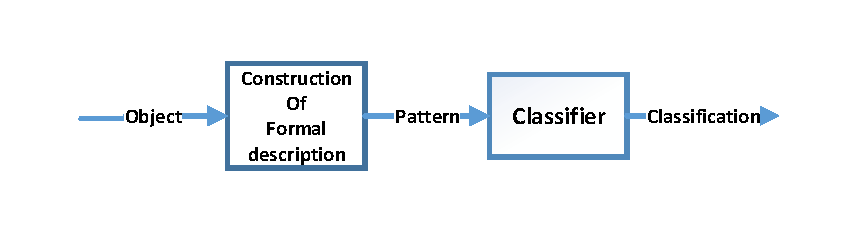
\includegraphics[width=0.8\textwidth]{graphics/pattern_recognition.pdf}
  \caption{Main pattern recognition steps \citep{obj_recogn_book}}
  \label{fig:pat_recog}
\end{figure}

It has been stated that no recognition can be done without some knowledge of the object to be recognised\citep[Page 381]{obj_recogn_book}. This knowledge is what specifies the properties that are to be recognised by the classifiers. Furthermore, the structure of how the knowledge is represented can be beneficial for how the pattern recognition is performed. In general pattern recognition is divided in two types; \textit{statistical} and \textit{syntactic}, which are described after knowledge representation is presented.\citep{obj_recogn_book}

\subsubsection{Knowledge Representation}\label{ssc:knowledge_representation}
There are many ways to represent the knowledge that is needed for pattern recognition and each representation can be used for any of the pattern recognition methods, however some representation methods are more beneficial for certain pattern recognitions, the two representations that are introduced here are mainly for statistical and syntactic recognition, respectively. 

\emph{Descriptions and features}

Even though descriptions are not considered pure knowledge representations, as they do not give a generalised representation, they can be used to represent some knowledge, as part of a greater, more complex structure \citep[Page 382]{obj_recogn_book}.
Features are representations of scalar properties, which can be used to describe object relations. To gather multiple descriptions for an object, \textit{feature vectors} are used. These feature vectors can in turn be used as input for statistical pattern recognition techniques.

An example of a feature vector can be of two features, \textit{compactness} (see \cref{ssc:heuristic_descr}), which can be used to determine the circularity of objects (perfectly round objects are the most compact), and a feature called \textit{size} which is used for describing the area of the given object. From these features a feature vector would be $x=(size, compactness)$. With definitions of what is small or big, and accepted circularity, the feature vector can then be used to classify objects as small, large, circular, non-circular and so forth.

\emph{Grammars and languages}

The description methods that were used to describe shapes, can also be used to describe objects. But to have the more general representation of an object class, these description methods are not sufficient. However, a way to classification is with the use of grammars and languages which is used in syntactic pattern recognition.


\subsubsection{Pattern recognition}\label{ssc:pat_recogn}
There are two main pattern recognition methods, statistical and syntactic. One big difference is that statistical pattern recognition mainly works with quantitative descriptions, whereas syntactical pattern recognition works with qualitative descriptions, and the knowledge representation they utilise differs.

\emph{Statistical pattern recognition}

Statistical pattern recognition often use features for knowledge representation. These features are used to make feature vectors, as explained in \cref{ssc:knowledge_representation}, that describe an object's properties. The collection of feature vectors used to describe objects in a class is called the feature space. Furthermore, classes of similar objects form clusters, which can be illustrated by a coordinate system, and in turn a function called a discrimination curve based on the properties, can be defined to separate these clusters so values greater than the discrimination curve will be members of one cluster and values below would be of the other cluster.

The classes are defined by statistical classifiers which each can take multiple inputs and only has one output. Each of these inputs take information about one of the features that are measured from the object under analysis. In this way different but similar objects from eg. a class of circular objects would all be recognised as circular objects, even though they are not identical.  \citep[Pages 387-404]{obj_recogn_book}.

\emph{Syntactic pattern recognition}

Syntactic pattern recognition often, but not necessarily use qualitative descriptions of objects and should be used when feature descriptions are not available or cannot be described. This is the case when objects are very complex or when an object can be represented as a hierarchical structure of simpler sub-regions.

Where statistical pattern recognition focused around features, the properties of objects in syntactical pattern recognition are called primitives. These primitives can be sub-regions of objects, and these objects of primitives can be described with graph or relational descriptions.
As explained in \cref{ssc:object_recognition}, the design of the descriptions are done by a designer in a non algorithmic manner based on experience and intuition. However, some guidelines have been defined to help the designer \citep[Page 410]{obj_recogn_book}:

\begin{enumerate}
\item The number of primitive types should be small
\item The primitives chosen must be able to form an appropriate object representation.
\item Primitives should be easily segmentable from the image
\item Primitives should be easily recognizable using some statistical pattern recognition method
\item Primitives should correspond with significant natural elements of the object (image) structure being described.
\end{enumerate}

Primitives can include line and curve segments, and relations between these primitives can be binary relations such as adjacent, left of, above, etc. This description structure can be compared to a structured natural language, representing knowledge as grammars and languages, as were described under \textit{Knowledge Representation}. Text in this language consists of sentences, which in turn consist of words and the words are constructed by letters that are concatenated and lastly it is these letters that correspond with primitives. Furthermore, the set of all letters are called an alphabet, and the set of words that can describe objects in a class is the description language which can describe all objects in the given class.\citep[Pages 410-418]{obj_recogn_book}.

\section{Object Recognition in Embedded Systems}
Since object recognition is a complex task, some issues may be introduced when performing recognition in an embedded system. Some of these issues are mentioned here. 

\emph{Big data sets}

Embedded systems have a limited amount of storage, which restricts both the size of images that can be analysed, but also how big a data stream the system would be able to handle, before the rate at which images arrive exceeds the rate at which the image can be handled.

\emph{Calculation speed}

The calculations that are done are heavy, as most recognition methods has to analyse all pixels in an image, and the computational power of embedded devices is restricted, which limits how many images that can be handled per second.

\emph{Camera quality and specialisation}
If the quality of images is low, noise in the images could be introduced and if the camera is not able to change focus automatically, objects too close or too far away will become blurry. Both issues can to some extend be handled with the use of dedicated tools, but it will require further calculations to be executed.

\section{Object Recognition Tool}\label{sc:ortool}
Object recognition is a complex task which can be solved with many existing tools \citep{cv_tools}. Because of the amount of tools, there are various different implementations and it is with great likelihood possible to find a tool that would solve the tasks of performing object recognition on the chosen hardware.

The tool that has been selected is \gls{opencv}\citep{opencv}. OpenCV has a number methods that can be used for recognition. The method that is used for this project is Template Matching, which matches a template image, which would be the object to be recognised, with a source image that is to be analysed which will be the images captured by the cameras that are used for the surveillance.

With the use of Template Matching it is possible to specify which pixel in the image is the center of the object that must be targeted. The following chapter explains how to utilize this.